\documentclass[12pt]{article}
\usepackage{anyfontsize}
\usepackage[a4paper, margin=2cm]{geometry}
\usepackage{polski}
\usepackage{tabto}
\usepackage{enumitem}
\usepackage{amsmath}
\usepackage{multirow}
\usepackage{multicol}
\usepackage{setspace}

\usepackage{listings}



\usepackage{tabularx}
\newcolumntype{C}{>{\centering\arraybackslash}X}
\newcolumntype{L}{>{\raggedleft\arraybackslash}X}
\newcolumntype{R}{>{\raggedright\arraybackslash}X}
\usepackage{wrapfig}

\usepackage{chngcntr}
\counterwithin{figure}{section}
\counterwithin{table}{section}
\numberwithin{equation}{section}

\usepackage{hyperref}
\hypersetup{
    colorlinks = true,
    urlcolor=blue,
    linkcolor= black
}

\usepackage{graphicx}
\graphicspath{{./Img/}}

\usepackage{csvsimple}
\usepackage{pgfplots}
\usepackage{pgfplotstable}
\pgfplotsset{compat= newest}


\usepackage{titlesec}
\titlelabel{\thetitle.\quad}
% \AddToHook{cmd/section/before}{\clearpage}

\usepackage[european, american currents, americanvoltages, RPvoltages, cute inductor]{circuitikz}
\usepackage{tikz}
\usetikzlibrary{shapes.geometric}
\ctikzset{
    logic ports=ieee,
    logic ports/scale=0.7,
}

\title{Dokumentacja projektu\\Gra z sterowaniem za pomocą protokołu TCP}
\author{Łukasz Przystupa}
\date{\today}

\usepackage{titling}
\renewcommand\maketitlehooka{\null\mbox{}\vfill}
\renewcommand\maketitlehookd{\vfill\null}

\begin{document}
    \begin{titlepage}
        \maketitle
        \thispagestyle{empty}
        \begin{center}
            Opiekun projektu: Jacek Kołodziej\\
            Przedmiot: Komunikacja między układowa
        \end{center}
    \end{titlepage}

    \section{Założenia projektowe}
    Celem projektu jest demonstracja działania protokołu TCP/IP. 
    Przetestowanie dwustronnej komunikacji oraz sprawdzenie jak działa komunikacja w czasie rzeczywistym.

    Projekt przedstawia prostą grę typu pong, w której gracz za pomocą wychyleń potencjometru steruje paletką.
    Sama komunikacja zaś opiera się na prostej zasadzie typu: pytanie odpowiedź.

\subsection{Metoda działania}
    \begin{figure}[!ht]
        \centering
        \begin{circuitikz}
            \draw
                (0, 0) node[draw, rectangle, minimum width = 2cm, minimum height = 2cm](MPU){MPU6050}
                (4, 0) node[draw, rectangle, minimum width = 2cm, minimum height = 2cm, align=center](CPU){Raspberry\\PICO}
                (10, 0) node[draw, rectangle, minimum width = 2cm, minimum height = 2cm](PC){PC}

                (MPU.east) ++ (0, 0.25) to[short, l = I2C] ++(1.9, 0)
                (MPU.east) ++ (0,-0.25) to[short] ++(1.9, 0)

                (6, 1.0) arc(60:-60:1)
                (7, 0.8) arc(60:-60:0.8)
                (8, 0.6) arc(60:-60:0.6)
                (7, 1.25) node[]{WiFi}
                (7,-1.25) node[]{TCP/IP}
            ;
        \end{circuitikz}
        \caption{Uproszczony model działania układu}
    \end{figure}
    Płytka Raspberry PI PICO W, jest pośrednikiem pomiędzy akcelerometrem MPU6050 a komputerem z uruchomionym serwerem gry.
    Mikrokontroler z jednej strony komunikuje się za pośrednictwem I2C z układem akcelerometru i żyroskopu MPU6050.
    Z drugiej zaś z pomocą bibliotek dostarczonych przez producenta oraz magistrali SPI z układem WiFi CWY43.
    Za pomocą tego układu nawiązywana jest komunikacja z hostem (komputerem z uruchomionym serwerem gry).

\subsection{Założenia funkcjonalne}
    Układ mikrokontroler powinien wykonywać dwa równorzędne zadania:
    \begin{enumerate}
        \item Odczytywać dane z akcelerometru,
        \item Monitorować stan TCP i w przypadku odebrania wiadomości odesłać aktualny stan akcelerometru.
    \end{enumerate}

    \begin{figure}[!ht]
        \centering
        \begin{circuitikz}
            \draw
                (0, 0) node[draw, circle, align=center](read){Odczytaj dane\\z akcelerometru}
                (0,-4) node[draw, circle, align=center](wait){Czekaj}

                (8, 0) node[draw, circle, align=center](TCP){Odpowiedz na\\wiadomości po TCP}
                (8,-4) node[draw, circle, align=center](blink){Mrugaj\\diodą}
            ;

            \draw[Stealth-, very thick] (read) to[bend left] (wait);
            \draw[Stealth-, very thick] (wait) to[bend left] (read);
            
            \draw[Stealth-, very thick] (blink) to[bend left] (TCP);
            \draw[Stealth-, very thick] (TCP) to[bend left] (blink);
        \end{circuitikz}
    \end{figure}

    \section{Testy funkcjonalne}
    Podczas pracy zostało stworzonych kilka podstawowych testów.
    Takich jak podstawowy test komunikacji z czajnikami, czy sprawdzenie działa połączenia po TCP.

    \subsection{Hardware -- I$^2$C}
        Sprawdzenie poprawności połączenia w przypadku czujników I$^2$C, należy do zadań prostych jednak niezwykle ważnych w przypadku prototypownia.
        Dlatego też autorka biblioteka opakowująca sterowaniem magistralą I$^2$C została wyposażona w funkcję \textit{I2C\_scan},

        \lstinputlisting[language=c, firstline=18, lastline=43, caption={Funckja sprawdzająca adresy dostępnych urządzeń}, label={listing:i2cScan}]{../pico/I2C/i2c.c}

        Listing \ref{listing:i2cScan} przedstawia funkcję \textit{I2C\_scan}, która sprawdza wszystkie możliwe adresy i wyświetla informację o znalezionych urządzeniach na standardowy wyjściu.
        Na zdjęcie 
        \begin{figure}[!ht]
            \centering
            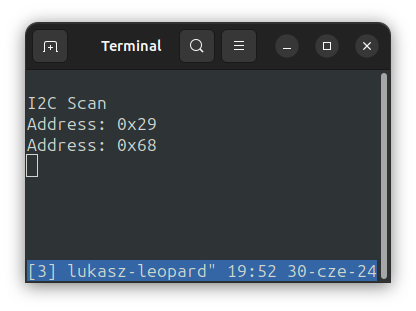
\includegraphics[height=0.12\textheight]{I2C_scan.png}
            \caption{Wynik działania funkcji \textit{I2C\_scan}}
        \end{figure}

    \subsection{Komunikacja między serwerem a klientem}
        W następnym teście sprawdzono poprawność komunikacji między serwerem a klientem.
        Mikrokontroler czytał aktualne wychylenie akcelerometru, następnie wysyłał dane na drugi rdzeń, gdzie po otrzymaniu prośby o następne dane, wysyłał je do serwera.
        \begin{figure}[!ht]
            \centering
            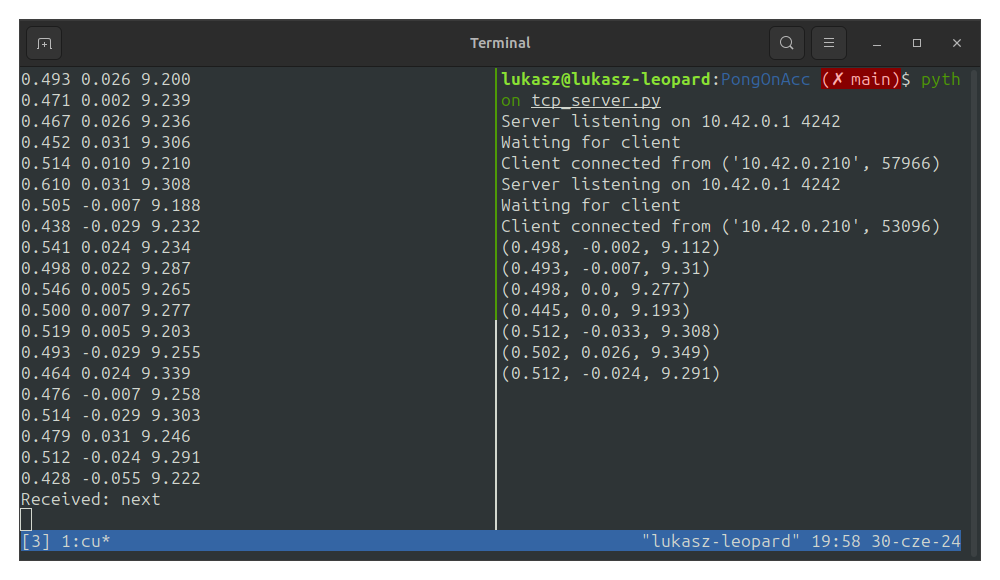
\includegraphics[width=0.7\textwidth]{TCP_test.png}
            \caption{Wynik działania testu komunikacji TCP}
        \end{figure}
    \section{Złożenie projektu}
    Ostatnim krokiem, było napisanie, prostej gry w języku Python.
    Wybraną grą był Pong -- prosta gra w której gracz za pomocą wychylania akcelerometry jest w stanie sterować ruchami paletki.
    Głównym powodem wyboru tej gry było, to że reakcje gracza muszą być interpretowane w czasie rzeczywistym, a wszystkie spowolnienia będą bardzo widoczne.
    \begin{figure}[!ht]
        \centering
        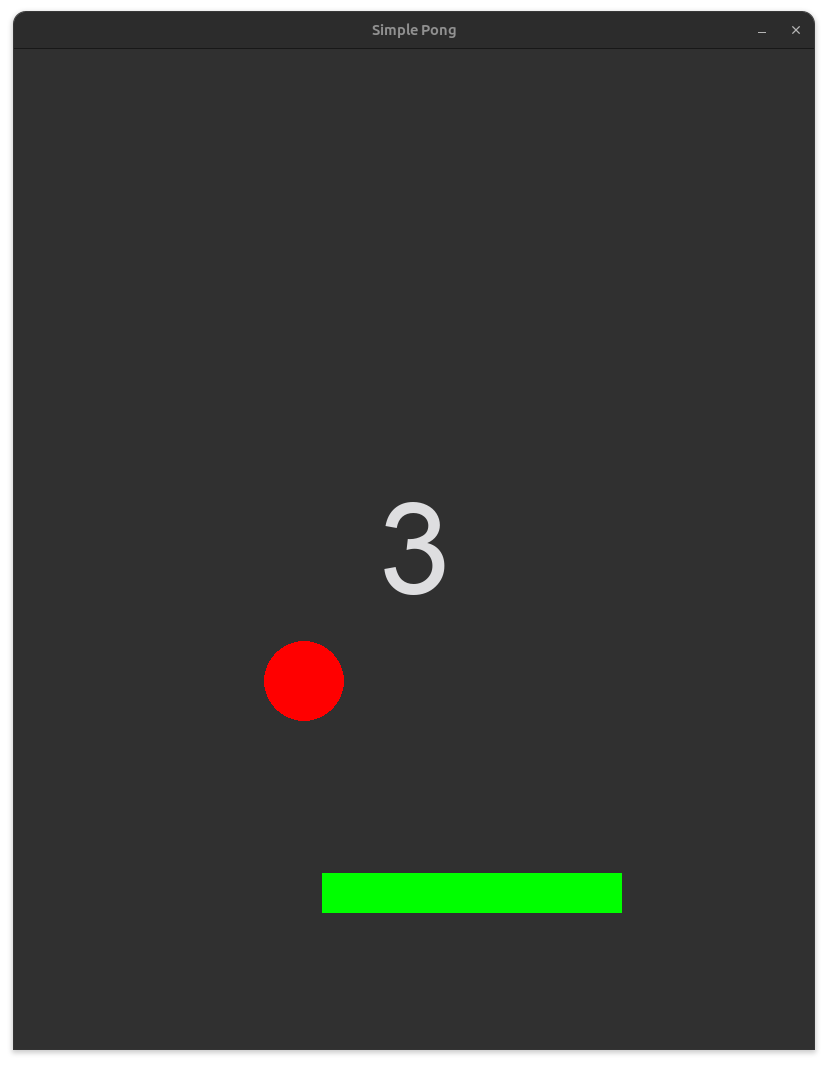
\includegraphics[width=0.4\textwidth]{pong.png}
        \caption{Gra Pong}
        \label{fig:pong}
    \end{figure}

    Rysunek \ref{fig:pong} przedstawia wyżej wymienioną grę z zaimplementowanym system sterowania ruchowego.

\section{Podsumowanie}
    Projekt zakończył się sukcesem, wszystkie założenia zostały spełnione.
    Jednak wykorzystanie standardu TCP do komunikacji w czasie rzeczywistym okazała się bardzo słabym wyborem.
    Aby układ pracował szybko oraz poprawnie, musiał został użyty jeden rdzeń na komunikację, zostawiający tylko jeden z dwóch dostępnych.
    Dodatkowo, okazyjnie zauważalne jest spowolnienie wynikające z tego że kontroler potrzebuje czasu aby odesłać odpowiedź do serwera.
    W mniej wymagającym czasowo scenariuszu, wykorzystane protokołu TCP może byś niezwykle użyteczne, a napisana biblioteka wykorzystana wielokrotnie.
    
    
    \vfill
    \begin{flushright}
        Łukasz Przystupa
    \end{flushright}
\end{document}
